This chapter is all about showing some nice tips and tricks to work productively using Ubuntu by harnessing the full potential of the Unity interface. It may be necessary to let go of old habits and cultivate new ones to make use of the features offered by Unity to work productively. The best way to remember these tips and tricks is to keep using them in your daily work schedule. There is never a better time to learn these tips than right now as  you read along this chapter. As usual, references are made to other operating systems to help ease the transition.

\section{Virtual Workspaces} \label{sect:virtual-workspaces} \index{Virtual Workspaces}
The desktop you perceive consists of the space offered by your physical screen size which could range from small sizes like $13^{\verb+"+}$ to big screens such as $27^{\verb+"+}$ or more. However imagine if you could increase this size virtually to increase the space to manage your applications in a more elegant fashion. This function is provided by virtual workspaces. The concept of virtual workspaces has been present in Ubuntu since its early conception dating back to its very first release Ubuntu 4.10 in the year 2004 despite only making a recent appearance in other operating systems such as Mac OS. Virtual workspaces can be invoked using the workspace icon located in the bottom left of the launcher or using the keyboard shortcut Super + S. The workspace icon looks like figure \ref{fig:workspace-icon}.

\begin{figure}[ht!]	
	\centering
	
\includegraphics[width=50pt]{./images/work-ubuntu/workspace-icon.png}
	\caption{Virtual Workspace icon}	
	\label{fig:workspace-icon}		
\end{figure}

\par \noindent On clicking the workspace icon or by pressing Super + S, the virtual workspaces (expo view) are shown as can be seen in figure \ref{fig:workspaces}. This provides a bird's view point of all the applications in all the workspaces. By default, there are four virtual workspaces. You can use workspaces to group applications to your liking. Imagine a scenario, where you place all work applications in workspace 1 while media and internet applications in the 2nd workspace. This way you can separately manage these applications. Applications can be moved to different workspaces easily either using keyboard shortcuts or by manually dragging applications from one workspace to the other. \\

\par \noindent Press the virtual workspace icon to get the expo view and from there you can manually drag and drop applications to any virtual workspace.  The other way of achieving this is by using keyboard shortcuts. Lets assume that you are in the top left workspace. To move an application you can then press Ctrl + Shift + Alt + Arrow Keys in the direction of the workspace you want to move it to. So to move an application to the top right workspace, you press Ctrl + Shift + Alt + Right Arrow Key and so on. The orange border indicates the currently focussed virtual workspace. To choose a particular workspace, double click it to enter into that workspace. \\

\par \noindent \framebox[6.7in][l]{\parbox[l]{6.5in}{\textbf{Tip}: You can increase the number of workspaces using 3rd party applications such as MyUnity which is explained in section \ref{sect:3rdpartyapps}.}} \\

\begin{figure}[ht!]	
	\centering
	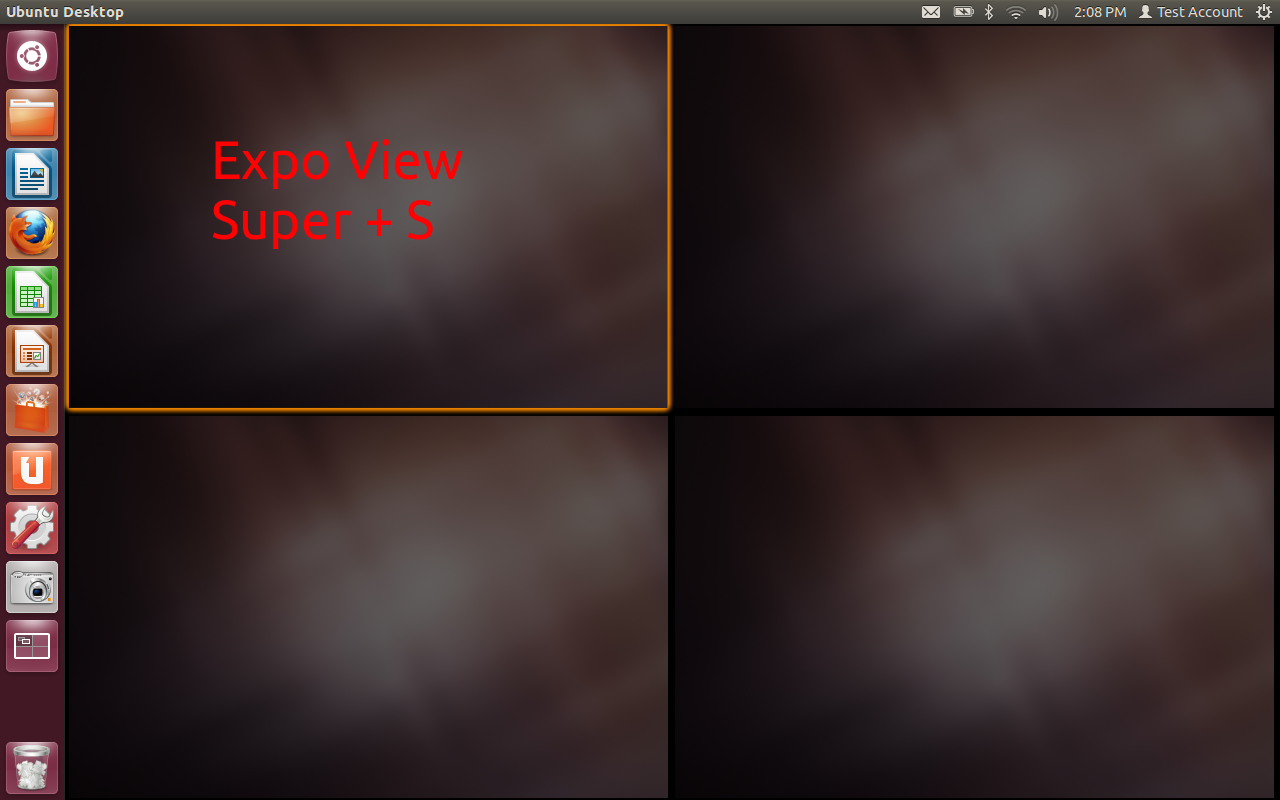
\includegraphics[width=325pt]{./images/work-ubuntu/workspaces.png}
	\caption{Virtual Workspaces}	
	\label{fig:workspaces}		
\end{figure}

\section{Switching between applications} \index{Switch between Applications}
Switching between applications in Ubuntu can be done in many ways to suit different situations. Let's look at two commonly used methods which is also used in other operating systems. 

\subsection*{Alt Tab} \index{Switch between Applications!Alt Tab}
The first method is by using Alt+Tab which is also commonly used in other operating system. So this shouldn't come as a surprise. You can switch between different application using Alt+Tab. When you press Alt+Tab, a pop up appears as seen in figure \ref{fig:alt-tab} where it shows all the applications open in that workspace. You can either press tab to switch to other application or you can also use the left or right arrow key. \\

\begin{figure}[ht!]	
	\centering
	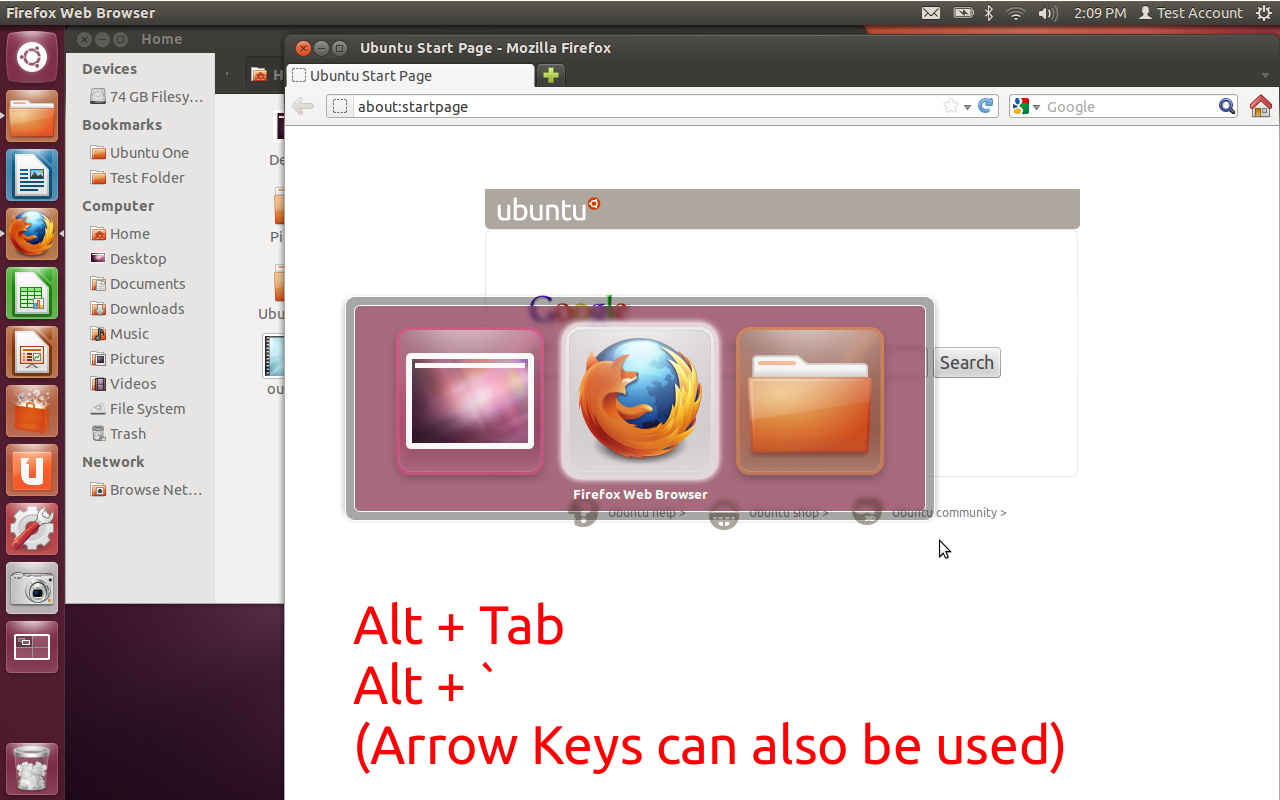
\includegraphics[width=325pt]{./images/work-ubuntu/alt-tab.png}
	\caption{Alt + Tab}	
	\label{fig:alt-tab}		
\end{figure}

\par \noindent There is one difference to be noted about Alt-Tab in Ubuntu and other operating systems. As you saw when you press Alt-Tab you can switch between \emph{different} applications with the emphasis on different. However, you want to switch between different instances of the \emph{same} application you should press Alt+\~ (grave, tilde) key. This will show previews of the different instances of the application currently focussed. In case your keyboard does not feature the tilde key above the tab key, Ubuntu maps the key directly above the tab key to achieve the same effect. This is to achieve consistent key bindings across different keyboard variants. When you press Alt + \~ (grave, tilde) you see a pop up similar to figure \ref{fig:alt-grave}. \\

\begin{figure}[ht!]	
	\centering
	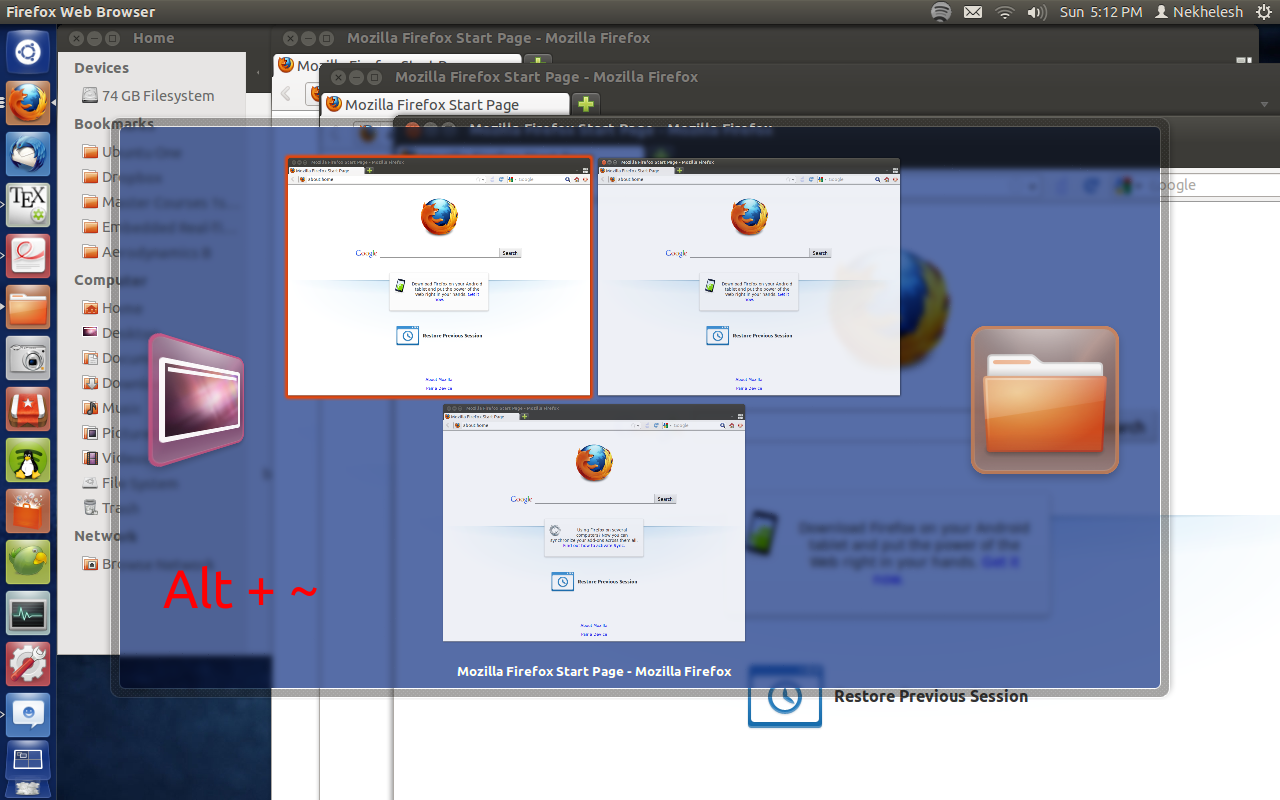
\includegraphics[width=325pt]{./images/work-ubuntu/alt-grave.png}
	\caption{Alt + (tilde, grave)}	
	\label{fig:alt-grave}		
\end{figure}

\subsection*{Spread view} \index{Switch between Applications! Spread View}
Another way of switching application is using the spread view option. The spread view can be activated by pressing Super + W. It will then show an overview of all the applications open in that workspace. This feature comes in handy when you have lots of application open. Instead of alt-tabbing through every one of them, you can activate the spread view and switch to that application directly by clicking on it in the spread view. This can be seen in figure \ref{fig:spread-view}. \\

\begin{figure}[ht!]	
	\centering
	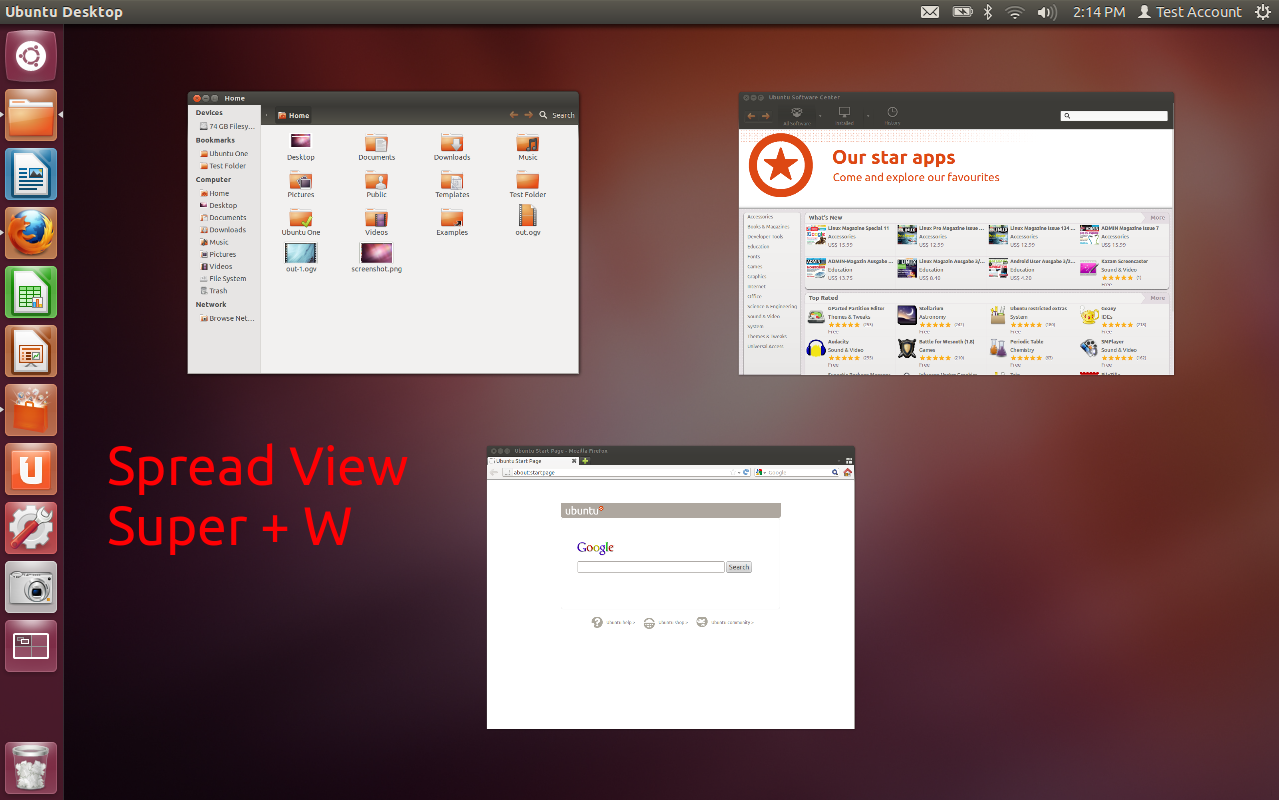
\includegraphics[width=325pt]{./images/work-ubuntu/spread-view.png}
	\caption{Spread View}	
	\label{fig:spread-view}		
\end{figure}

\section{Heads Up Display (HUD)}
The Heads Up Display has already been described in detail in section \ref{sect:desktop-hud}. The purpose of mentioning it again is to recollect about how the HUD can improve the experience with dealing with the menu structure. The same example with the Firefox application is again briefly repeated. Instead of having to manually through the menu structure for a particular option you are looking for, you can get it much quicker using the HUD. The HUD can be activated by pressing the Alt key. 

\section{Keyboard shortcuts for using Unity} \index{Switch between Applications!Keyboard Shortcuts}
If you haven't realised the golden rule of working productively on a computer, well here it is. The golden rule to working productively on your computer is by using a combination of keyboard shortcuts and the mouse. Unity offers a complete suite of keyboard shortcuts to achieve every little work task you want to perform. Right from switching between workspace, application to launching applications, there are keyboard shortcuts for every one of them. The best part of this is that you do not need to remember them all at once. You will automatically get a hang of it as you start using Ubuntu. Meanwhile, at the start you can use the keyboard shortcut overlay to your advantage to see all the available shortcuts. You can activate the keyboard shortcut overlay (pop up) by holding on Super for a few seconds. You will then see number overlay on the launcher icons as seen in figure \ref{fig:number-overlay}. \\

\begin{figure}[ht!]	
		\centering		
		\subfloat[]
		{ 	\label{fig:sound-menu} 	
\includegraphics[width=40pt]{./images/work-ubuntu/number-overlay1.png} } 
		~ \hspace{0.5in}
		\subfloat[]
		{ 	\label{fig:messaging-menu} 
\includegraphics[width=40pt]{./images/work-ubuntu/number-overlay2.png}	}
		~ \hspace{0.5in}
		\subfloat[]
		{ 	\label{fig:messaging-menu} 
\includegraphics[width=40pt]{./images/work-ubuntu/number-overlay3.png}	}
		~ \hspace{0.5in}
		\subfloat[]
		{ 	\label{fig:messaging-menu} 
\includegraphics[width=40pt]{./images/work-ubuntu/number-overlay4.png}	}		
		\caption{Number overlay}
		\label{fig:number-overlay}
\end{figure}

\par \noindent \framebox[6.7in][l]{\parbox[l]{6.5in}{\textbf{Tip}: You can launch application shown in the launcher using the help of the number overlay. For instance in figure \ref{fig:number-overlay}, you can launch Firefox by pressing Super + 3. Similarly you can launch other applications in the launcher using Super + Number keyboard shortcut.}} \\

\par \noindent You will also see a keyboard shortcut overlay as can seen be in figure \ref{fig:shortcut-overlay}. As already mentioned before, this shortcut overylay shows all the available keyboard shortcuts that you need to know to work productively. \index{Keyboard Shortcut Overlay} \\

\begin{figure}[ht!]	
	\centering
	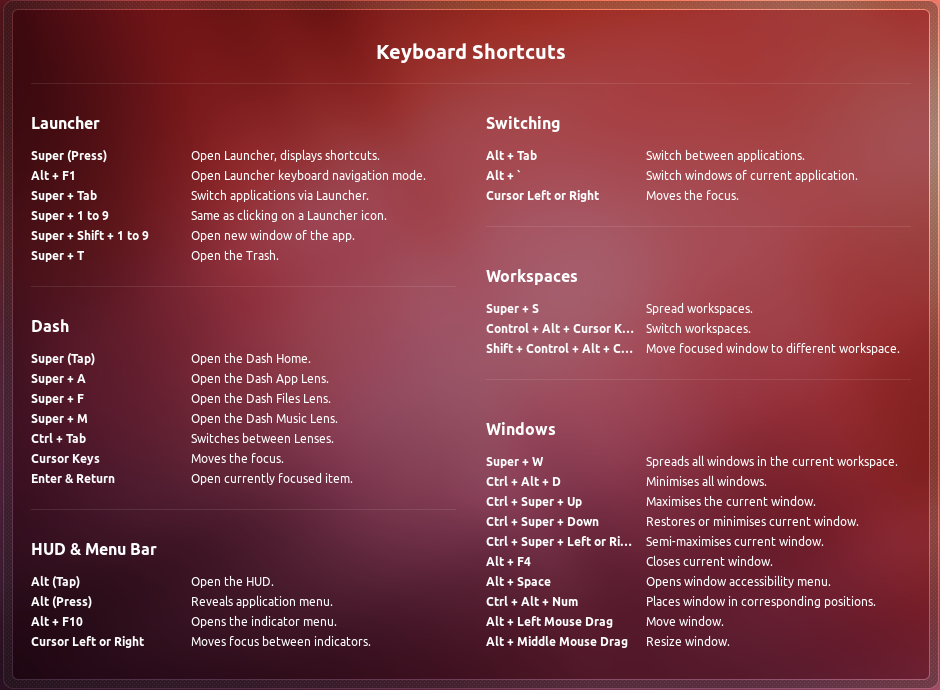
\includegraphics[width=325pt]{./images/work-ubuntu/shortcut-overlay.png}
	\caption{Keyboard Shortcut overlay)}	
	\label{fig:shortcut-overlay}		
\end{figure}